\section{Execution Model}
This section discusses the execution model of the virtual machine using
a refinement strategy. Starting from an overview, it is shown how scheduling
is organized. Upon this, a single interpreter model is introcued.
This simplified model
is then successivly refined until full parameterisation over
interpreters is achieved.
\subsection{Overview}
\begin{figure}[ht]
\centering
\includegraphics[width=9cm]{figures/exec_overview.eps}
\caption{\label{model_overview} {\it Simplified execution model}}
\end{figure}

Figure \ref{model_overview}
shows the simplified execution model of the virtual machine.
Its main parts are the scheduler,
the worker and a construct called interpreter.

Every execution in the machine is controlled by the scheduler which assigns
threads to a worker.
The worker then executes the thread using the interpreter.

Depending on the state of computation, control is passed
forth and back to the worker and scheduler.
\subsection{Scheduling work}
\begin{figure}[ht]
\centering
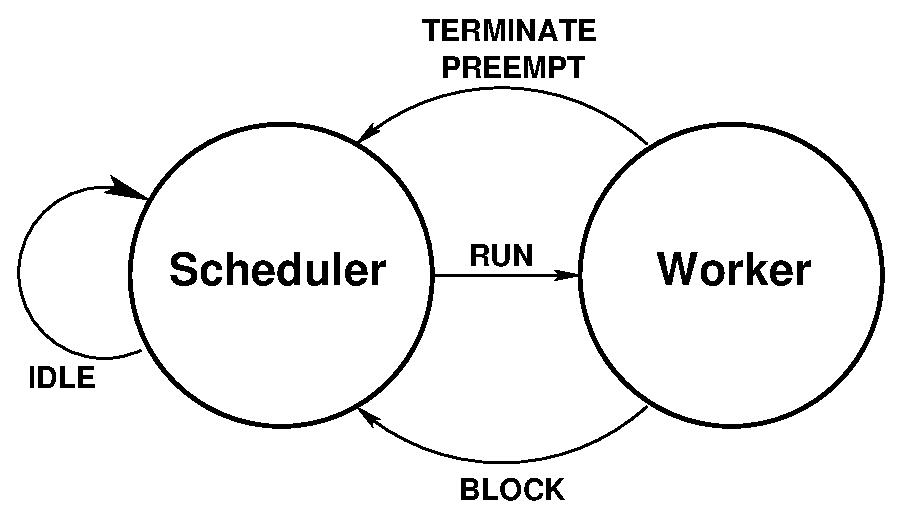
\includegraphics[width=6cm]{figures/exec_scheduler.eps}
\caption{\label{model_scheduler} {\it Scheduler-Worker interaction}}
\end{figure}

The {\em scheduler} is reponsible for the fair and preemtive scheduling
of threads (cf. figure \ref{model_scheduler}).
When no runnable thread exists, the scheduler runs in the
{\em idle loop}, waiting for I/O. When one or more threads are runnable
the scheduler selects one using a fair strategy and invokes the worker
to execute this thread.

The {\em worker} executes a single thread until it is finished, the
preemption condition is reached or computation blocks due to an unbound
transient.

In these cases control is passed back to the scheduler
which then trys to select a new thread for execution.
If this fails and no I/O is waiting,
the machine terminates since no computation is left.

The message {\em block} also has the side effect that the
blocking thread is added to the
wait queue of the transient it blocks on.
\subsection{A single interpreter}
\begin{figure}[ht]
\centering
\includegraphics[width=6cm]{figures/exec_interpreter.eps}
\caption{\label{model_interpreter} {\it Worker-Interpreter interaction}}
\end{figure}

A thread contains tasks, which are executed sequentially following
a stack discipline.
A {\em task} provides the bytecode to be executed by the interpreter.

The worker executes the tasks and sents a {\em run}
message to the interpreter.

The {\em interpreter} (cf. figure \ref{model_interpreter}) sequentially executes
the instruction of the code indicated with
the {\em next} message until one of the following conditions is reached:
\begin{itemize}
\item
it finished the topmost task on the stack ({\em continue}),
\item
a new task was created ({\em push}),
\item
the value of an unbound transient is needed ({\em request}),
\item
until an exeption was raised ({\em raise}).
\end{itemize}
In these cases control is passed back to the worker.

In case of {\em continue}, the worker
pops the current task and  continues executing the
new topmost task on the task stack.

In case of {\em push}, the worker
pushes the new task to the stack and starts executing it.

In case of {\em request}, control is passed to the scheduler with message
{\em block} to have the thread added to the wait queue of the transient
it blocks on.

In case of {\em raise}, the worker sents a {\em handle} message
to the intepreter. {\em handle} behaves the same as {\em run}
in that it returns the same results as the {\em run} message.
\subsection{Multiple interpreters}
The single interpreter model is now parameterized over the interpreter.

The key idea is that he interpreter
is no longer hard-wired in the system.
Instead, it can be plugged in on demand during runtime.

The system knows nothing about a interpreter but the generic
interpreter interface shown in figure \ref{model_interpreter}.
All operations are invoked using this interface.

The only price to pay for is that tasks need to be parameterized over
the interpreter. Each time the worker executes a task
it now firsts extracts the interpreter the task belongs to and
sents this interpreter either the {\em run} or {\em handle} message.

Interpreter parameterisation yields the following strong properties:
\begin{enumerate}
\item
System services such as pickler and unpickler can be expressed using
interpreters. This allows for infrastructure sharing and thus simplifies
the machine while retaining the same level of expressivity.
\item
Each language can provide different interpreters for different purposes,
such as memory efficient execution, fast execution, or debug execution.
\item
The machine can host several co-existing languages very easily.
\end{enumerate}
\begin{paragraph}{Language interoperability.}
To achieve language interoperability on closure level, it is sufficient
to addionally parameterize closures over the interpreter. This
requires closures to be part of the abstract data layer.

Provided that the intersection of the LDLs is not empty, the languages
can interoperate on this subset for free.
\end{paragraph}
